\subsection{Ground station networks}

Ukjent nettverk
Ukjente deltakere
Ukjent utstyr



\subsubsection{NTNU and Aalborg University}
Simulating a network consisting of NTNU and Aalborg University is interesting, since Aalborg University are the developers of the BlueBox satellite network.
\begin{figure}
  \begin{center}
    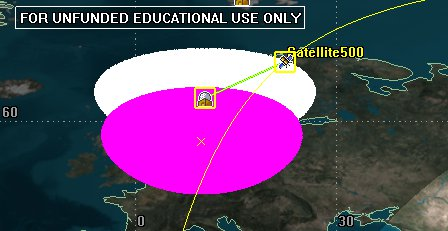
\includegraphics[width=0.7\textwidth]{Figures/range_ntnu_aalborg}
  \end{center}
  \caption[NTNU Aalborg]{Ground station network: NTNU and Aalborg}
  \label{fig:range_ntnu_aalborg}
\end{figure}

A ground station network consisting of NTNU and Aalborg University is not very efficent, see Fig. \ref{fig:range_ntnu_aalborg}.

\subsubsection{NTNU and UNIS}
 
\begin{figure}
  \begin{center}
    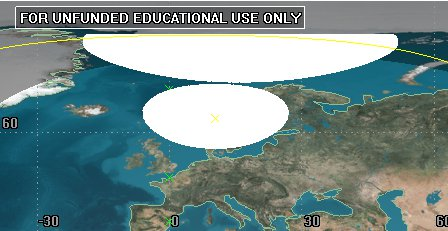
\includegraphics[width=0.7\textwidth]{Figures/range_ntnu_svalbard}
  \end{center}
  \caption[NTNU Aalborg]{Ground station network: NTNU and UNIS}
  \label{fig:range_ntnu_unis}
\end{figure}